In this section we explore the effect of varying the underlying binary physics assumptions, both on the detection rate (Section~\ref{sec:detection_rate_analysis}) and the properties of the detectable systems (Section~\ref{sec:property_variations}).

\subsection{Detection rates}\label{sec:detection_rate_analysis}
In Figure~\ref{fig:detection_rates}, we show the expected number of LISA detections for each model variation and discuss the prominent trends in the following sections. For the exact rates and uncertainties plotted in this figure see Table~\ref{tab:detection_rates} and for a plot of the rates relative to the fiducial model see Fig.~\ref{fig:dco_relative_rates}.

The BHBH detection rate is markedly robust across variations of physics assumptions, as can be seen in the top panel of Figure~\ref{fig:detection_rates}, with the mean detections in three quarters of our models staying within 25\% of the fiducial rate. In contrast, the BHNS detection rate is very sensitive to all changes that we made in our binary physics assumptions, varying across two orders of magnitude in the middle panel of Figure~\ref{fig:detection_rates}. Finally, in the last panel of Figure~\ref{fig:detection_rates} we show that the NSNS detection is only moderately sensitive to certain changes in physics assumptions, varying by up to an order of magnitude, whilst showing no change for many models.

\subsubsection{Mass transfer variation trends}

In models \modBetaLow{}-\modBetaHigh{}, we set the mass transfer efficiency $\beta$ to a fixed value. For the BHBHs and BHNSs, as we increase $\beta$ the detection rates steadily decrease. This may seem unintuitive since one might assume that a higher mass transfer efficiency would lead to more massive compact objects and thus a more detectable population. However, this increase contributes to the envelope mass and so without increasing the core mass or fallback rate, the final compact object mass is relatively unaffected. Moreover, one must consider that most of these DCOs are formed through a common-envelope event and so retaining more of the envelope during mass transfer means that the eventual ejection of the envelope is much more difficult, thus leading to more stellar mergers and fewer detectable systems \citep[e.g.][]{Kruckow+2018,Broekgaarden+2021}.

In contrast, for the NSNSs, the detection rate increases with increasing $\beta$. This is for two main reasons: firstly the ejection of a common-envelope is less problematic for NSNSs as they are less massive \citep[e.g.][]{Kruckow+2018}. Moreover, the increased mass transfer efficiency means that systems that were previously below the mass necessary to become a NS can now accrete enough mass to form a NS. Although the same is true for more massive stars becoming BHs instead of NSs, due to the IMF, there is a net flux of more stars becoming NSs.

Enforcing that case BB mass transfer is always unstable (model \modCaseBB{}) has little effect on the BHBH detection rate whilst moderately and drastically decreasing the detection rates of BHNSs and NSNSs respectively. This is because a large fraction of NSs (and the majority of NSNS binaries) are formed through case BB mass transfer. Therefore, setting this mass transfer to be always unstable results in many of these binaries to merge before they could become DCOs since we assume the pessimistic common-envelope (CE) scenario by default.

If we instead use the optimistic CE scenario when setting case BB mass transfer to be unstable (model \modCaseBBOpt{}) we find that the rates instead uniformly increase across DCO types. This is both from the natural increases from using the optimistic CE scenario (see discussion of model \modOpt{} in Sec.~\ref{sec:detection_rate_CE_trends}), as well as additional increases from adding more DCOs formed through CE events after case BB mass transfer. This explains why we see more detections for BHNSs and NSNSs in model \modCaseBBOpt{} than in model \modOpt{}.

\begin{figure*}[p]
    \centering
    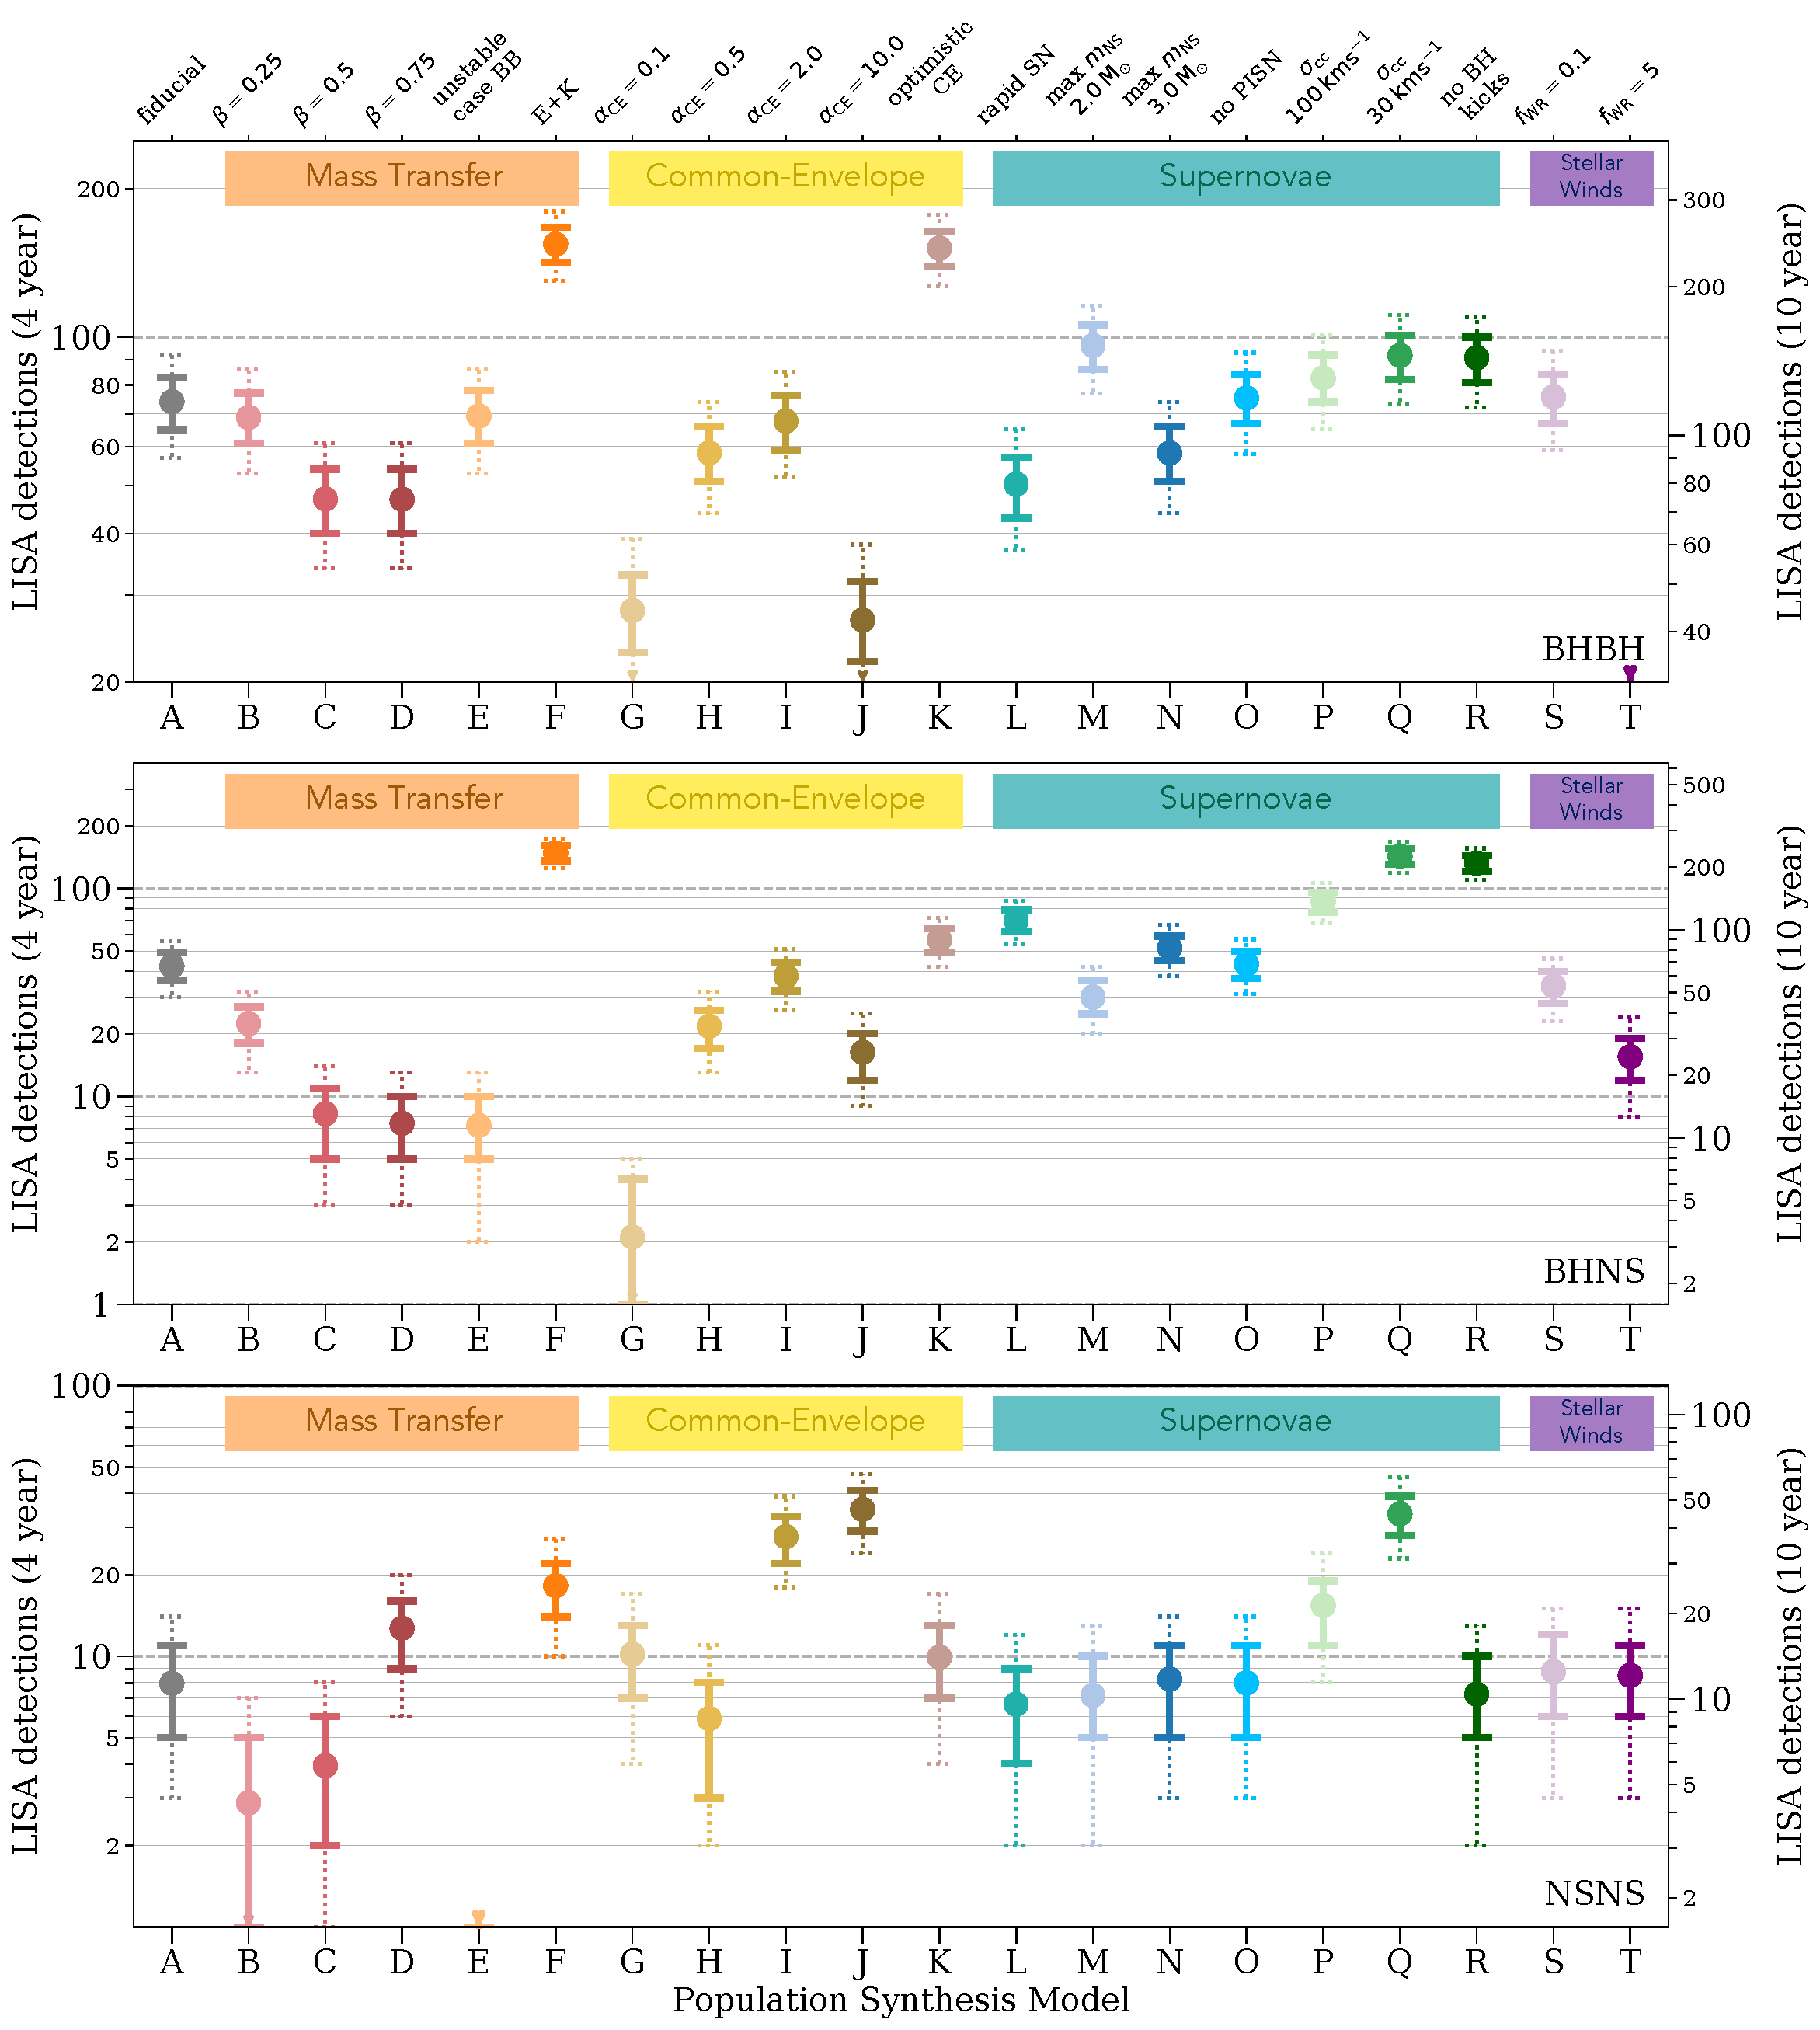
\includegraphics[width=\textwidth]{fig7_dco_detections.pdf}
    \caption{The number of expected detections in the LISA mission for different DCO types and model variations. Error bars show the 1- (solid) and 2-$\sigma$ (dotted) Poisson uncertainties. An arrow indicates that the error bar extends to zero. The left axis and grid lines show the number of detections in a 4-year LISA mission and the right axis shows an approximation of the number of detections in a 10-year mission (we scale the axis by $\sqrt{T_{\rm obs}}$, see Table~\ref{tab:detection_rates} for exact rates). Each model is described in further detail in Table~\ref{tab:physics_variations} and details of the fiducial assumptions are in Section~\ref{app:fiducial_physics}. See also Fig.~\ref{fig:dco_relative_rates} and Sec.~\ref{sec:detection_rate_analysis} for a discussion. \href{https://github.com/TomWagg/detecting-DCOs-in-LISA/blob/main/paper/figures/fig7_dco_detections.png}{\faFileImage} \href{https://github.com/TomWagg/detecting-DCOs-in-LISA/blob/main/paper/figure_notebooks/variations.ipynb}{\faBook}.}
    \label{fig:detection_rates}
\end{figure*}

\subsubsection{Common-envelope variation trends}\label{sec:detection_rate_CE_trends}

Models \modAlphaLowest{}-\modAlphaHighest{} alter $\alpha_{\rm CE}$, the common-envelope efficiency parameter, to $0.1, 0.5, 2.0$ and $10.0$ respectively (where the fiducial model has $\alpha_{\rm CE} = 1.0$). Although we see that there are large variations in the LISA detection rates when changing $\alpha_{\rm CE}$, the detectable \textit{fraction} of systems remains largely unchanged. Therefore, any changes in the detection rate are due to changes in the \textit{formation} rate of the DCOs.

Altering $\alpha_{\rm CE}$ has two major effects on the formation rate of double compact objects. Recall that $\alpha_{\rm CE}$ represents the fraction of the orbital energy that is available for the ejection of the common-envelope. Therefore, increasing $\alpha_{\rm CE}$ allows common-envelope ejection to occur at larger separations (since more energy is available at any given separation). A second effect of increasing $\alpha_{\rm CE}$ is that common-envelopes are less likely to result in stellar mergers as more energy is available for envelope ejection. We can understand the trends in formation rate of the three DCO types by considering these two effects.

The BHBH rate peaks for $\alpha_{\rm CE} = 1$ (model \modFid{}) and reduces whether we increase \textit{or} decrease $\alpha_{\rm CE}$. This is because the increase in $\alpha_{\rm CE}$ shifts a significant fraction of the population to such large separations that they no longer merge within a Hubble time. Although the number of stellar mergers decreases as well, the overall change in the merging BHBH formation rate is negative. The inverse is also true for decreasing $\alpha_{\rm CE}$, where BHBHs have shorter separations but stellar mergers are more frequent. Thus we find that $\alpha_{\rm CE} = 1$ seems to be optimal for BHBHs by balancing these two effects most effectively.

The BHNS rate follows the same pattern as BHBHs. This is expected since the BH is formed first for every BHNS in our sample and so the common-envelope event is due to a RLOF of BH progenitor, just as with BHBHs. However, given the similarity in the BHNS rates between $\alpha_{\rm CE} = 1$ and $\alpha_{\rm CE} = 2$ (models \modFid{} and \modAlphaHigh{}), the `optimal' $\alpha_{\rm CE}$ for BHNSs seems to be somewhere between 1 and 2 rather than very close to 1 as with BHBHs.

In contrast, $\alpha_{\rm CE} = 1$ is far from optimal for NSNSs. Increasing $\alpha_{\rm CE}$ (models \modAlphaHigh{} and \modAlphaHighest{}) results in significantly higher rates. This is because LISA detectable NSNSs tend to have been formed very recently before detection (see Fig.~\ref{fig:fiducial_pdf_distributions}e). Therefore, though higher $\alpha_{\rm CE}$ results in larger \textit{initial} separations, this does not adversely affect the NSNS rate as the systems are simply detected later after their formation compared to the fiducial model. So for models \modAlphaHigh{} and \modAlphaHighest{}, fewer systems result in stellar mergers and the overall population remains within the LISA band, producing much higher detection rates. %Finally, for model \modAlphaLowest{}, the reduction in common-envelope efficiency is strong enough that a sufficient number of systems are formed at shorter separations to offset those lost to stellar mergers.

We explore the optimistic CE scenario in model \modOpt{}, meaning that we allow Hertzsprung gap donors to survive CE events. A large fraction of the progenitors of the BHs in our sample expand significantly during the Hertzsprung gap phase and initiate CE events. This means that, when we assume the optimistic CE scenario, the formation rate of BHs is greatly increased. Therefore, similar to models \modAlphaLowest{}-\modAlphaHighest{}, we find that though the detectable \textit{fraction} does not change significantly, the increased formation rate of BHs in the Milky Way leads to this model predicting significantly more BHBH detections.

The progenitors of BHNSs tend to be less massive than those of BHBHs. Less massive stars expand less during the Hertzsprung gap and thus initiate CE events less frequently in this phase. For these reasons, as can be seen most clearly in Fig.~\ref{fig:dco_relative_rates}, the relative increase in model \modOpt{} compared to the fiducial model is lower than BHBHs for BHNSs. For the same reason, the NSNS detection rate shows little significant change.

\subsubsection{Supernova variation trends}

Changes to the remnant mass prescription (models \modRapid{}-\modNSHigh{}) have no effect on the NSNS detection rate for two reasons. A large fraction of the NSs in our sample are formed through ECSN, in which case their masses are set to $1.26 \unit{M_\odot}$ regardless of the remnant mass prescription. Secondly, the majority of the remaining NSs have such low progenitor masses that they are set to the lowest remnant mass in the prescription ($1.28 \unit{M_\odot}$ for the delayed prescription and $1.1 \unit{M_\odot}$ for the rapid prescription). This means that changing the upper portion of the mass range of NSs in the remnant mass prescription has little effect.

This is not the case for BHBHs and BHNSs. The different remnant mass prescriptions and maximum neutron star masses change whether a progenitor becomes a black hole or a neutron star. Hence, using the rapid prescription (model \modRapid{}) or increasing the maximum neutron star mass (model \modNSHigh{}), means that more progenitors form high mass NSs rather than low mass BHs and so more BHNSs are formed. This explains the higher detection rates for BHNSs and lower detection rates for BHBHs in these models. The inverse is true for model \modNSLow{}, where instead more BHBHs are formed and detected.

Additionally, we find that not implementing pair-instability supernovae (PISN) pulsational pair-instability supernovae (PPISN) in model \modNoPISN{} has no effect on the results for any DCO type. This is because the average metallicity of the Milky Way is high enough than no progenitor retains enough mass to initiate a PISN or PPISN.

Decreasing the core-collapse supernova velocity dispersion (models \modSigLow{}-\modSigLower{}) increases the detection rates for each DCO type since lower kicks result in fewer disrupted binaries and hence a more numerous detectable population. This increase is least prominent for BHBHs since their increased mass mean that disruptions are less frequent than, for instance, in NSNSs. It is also notable that these two models best match the detection rates from LIGO (Broekgaarden et al.\ in prep). Therefore we find the best matching models for the LIGO detection rates also produce the highest LISA detection rates.

In model \modNoBH{} we do not give black holes natal kicks. For BHBHs, the rate is approximately equal to that of model \modSigLower{} since kicks of $30 \unit{km}{s^{-1}}$ are equivalent to no kicks for massive BHs in our sample. For BHNSs, this model's rate is still well above the fiducial but decreases slightly relative to model \modSigLower{} as the number of surviving binaries is limited by the neutron star kick more than the black hole kick. NSNSs are unaffected as one would assume due to the absence of BHs.

\subsubsection{Stellar wind variation trends}
We decrease the efficiency of Wolf-Rayet winds to 10\% in model \modWRLow{}. We find that decreasing the efficiency of these winds actually has very little effect on our predicted detection rates. This due to a combination of cancelling effects.

Firstly, the decreased winds mean that the DCOs (particularly those containing BHs) are generally more massive and so more detectable in LISA. Secondly, one may expect that LISA sources in model \modWRLow{} would be higher frequency than in our fiducial model as decreased winds generally result in tighter binaries. However, though this \textit{is} the case at DCO formation, we find by the time the sources have evolved until the LISA mission they are actually at \textit{lower} frequencies than in our fiducial model. This is because the reduced winds allow DCOs to be formed at higher metallicity and, therefore, at more recent times. This means that the DCOs do not evolve for as long before the LISA mission and so remain at lower frequencies (wider separations) thus making them less detectable. Finally, we find that NSNSs are more eccentric and BHBHs are less eccentric than our fiducial model (with BHNSs relatively unchanged). The increase in eccentricity for NSNSs comes from the same reason as the lower frequency, more recent birth times mean that binaries have less time to circularise. The same is not true for BHBHs as the more massive systems are less affected by supernova kicks and so fewer high eccentricity systems are formed.

Overall, despite the large differences in the system properties, these three effects in combination leave the detection rates relatively unchanged.

In model \modWRHigh{} we instead \textit{increase} the efficiency of Wolf-Rayet winds by a factor of 5. In this model the detection rate of BHBHs decreases by over a factor of 10 and BHNSs by over a factor of 2 whilst the NSNS rate is relatively unchanged. Increasing the efficiency of WR winds strongly decreases the final masses of DCOs. This means that many progenitors that would have formed LISA sources under our fiducial assumptions would not have enough mass to produce a DCO, or produce a NS instead of a BH (therefore this effect is stronger on BHBHs than NSNSs). Moreover, DCOs that are formed tend to be less massive and therefore less detectable.

\subsection{Properties of detectable systems}\label{sec:property_variations}

In this section, we consider how varying underlying physics assumptions changes the properties of detectable systems. We focus on several key differences across physics variations rather than showing the differences in every model and thus this section is by no means exhaustive.

\subsubsection{Using LISA to investigate the lower mass gap}\label{sec:lower_mass_gap}

\begin{figure}[tb]
    \centering
    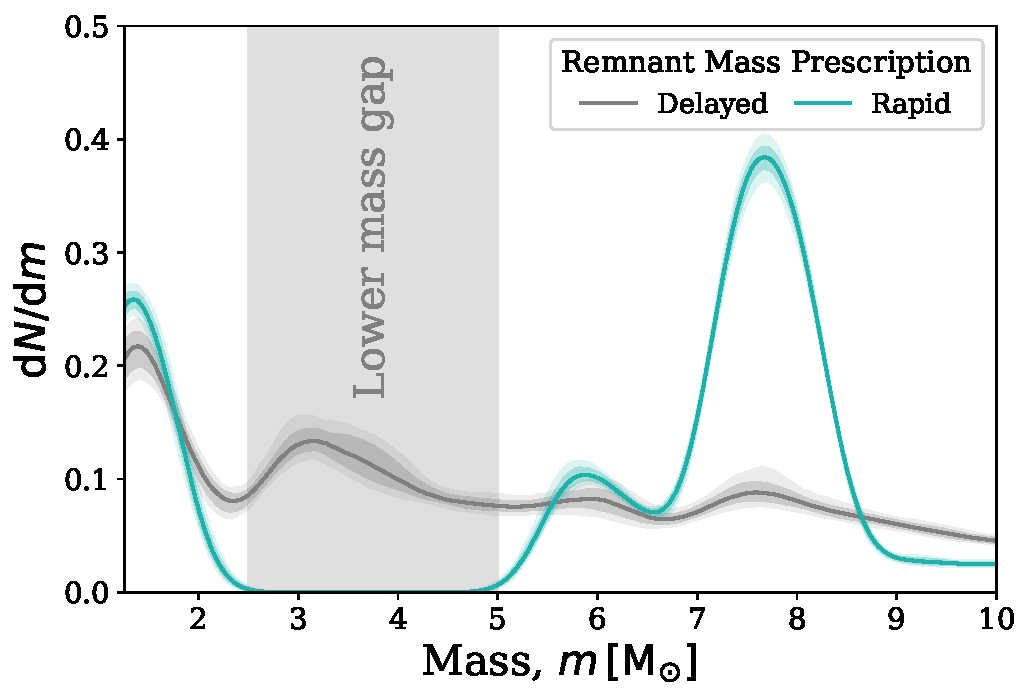
\includegraphics[width=\columnwidth]{fig8_lower_mass_gap_rapid_variation.pdf}
    \caption{Comparison of the component mass distribution of LISA detectable DCOs when using the Fryer delayed (model \modFid{}) and rapid (model \modRapid{}) remnant mass prescriptions. Distributions are plotted in the same way as Fig.~\ref{fig:fiducial_pdf_distributions}, except all DCOs types are shown in one curve and each type is weighted by its detection rate in the respective model. \href{https://github.com/TomWagg/detecting-DCOs-in-LISA/blob/main/paper/figures/fig8_lower_mass_gap_rapid_variation.pdf}{\faFileImage} \href{https://github.com/TomWagg/detecting-DCOs-in-LISA/blob/main/paper/figure_notebooks/variations.ipynb}{\faBook}.}
    \label{fig:lower_mass_gap_variation}
\end{figure}

In Figure~\ref{fig:lower_mass_gap_variation}, we show the component mass distribution for all LISA detectable DCOs (BHBHs, BHNSs and NSNSs) for two different remnant mass prescriptions. The grey distribution uses the Fryer \textit{delayed} remnant mass prescription \citep{Fryer+2012}, which is our fiducial assumption (model \modFid{}). This prescription produces compact objects in the lower mass gap ($2.5 \unit{M_{\odot}} \le m \le 5 \unit{M_{\odot}}$) and indeed we find that, of the LISA detectable DCOs, approximately \BHBHatLeastOneLowerMassGapPerc{}\% of BHBHs, \BHNSatLeastOneLowerMassGapPerc{}\% of BHNSs and \NSNSatLeastOneLowerMassGapPerc{}\% of NSNSs have at least one component in the lower mass gap. Overall, weighting by the relative detection rates, this gives that 55\% of our predicted LISA DCO detections would have at least one component in the lower mass gap when using this remnant mass prescription.

Alternatively, the blue curve in Fig.~\ref{fig:lower_mass_gap_variation} shows the same distribution but for the \textit{rapid} remnant mass prescription \citep{Fryer+2012}, which we use in model \modRapid{}. In this case, no compact objects are formed (and therefore, detected) in the lower mass gap. From the stark difference between these models, it is clear that it is difficult at this point to say with any certainty what fraction of systems LISA will detect in the lower mass gap given the highly uncertain formation rate of systems in this mass range.

However, it is important to highlight that \textit{if} DCOs are formed with components in the lower mass gap, LISA \textit{will} be able to detect them. And thus, LISA could be a useful instrument for providing evidence for the existence or non-existence of a lower mass gap based on the mass distribution of detected DCOs.

\subsubsection{Effect of natal kicks on eccentricity distribution}

\begin{figure}[tb]
    \centering
    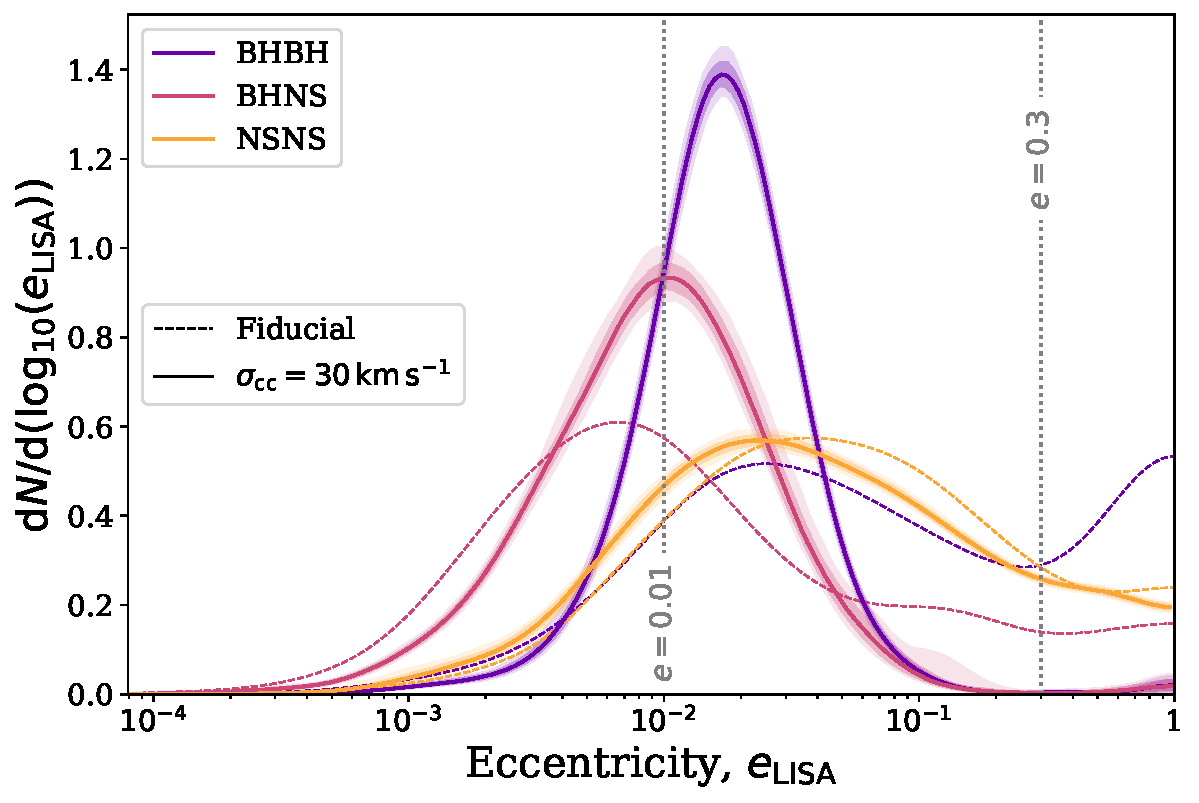
\includegraphics[width=\columnwidth]{fig9_ecc_low_kick_variation.pdf}
    \caption{As Fig.~\ref{fig:fiducial_pdf_distributions}d, but for model \modSigLower{}. For comparison, we show the mean distribution for the fiducial model (model \modFid{}) as dashed lines. \href{https://github.com/TomWagg/detecting-DCOs-in-LISA/blob/main/paper/figures/fig9_ecc_low_kick_variation.pdf}{\faFileImage} \href{https://github.com/TomWagg/detecting-DCOs-in-LISA/blob/main/paper/figure_notebooks/variations.ipynb}{\faBook}.}
    \label{fig:ecc_low_kick_variation}
\end{figure}

In Figure~\ref{fig:ecc_low_kick_variation}, we investigate how decreasing the magnitude of natal kicks from core-collapse supernovae affects the eccentricity distribution of LISA detectable DCOs. For reference, we show the mean fiducial distributions (model \modFid{}) as dashed lines (see Fig.~\ref{fig:fiducial_pdf_distributions}d for full comparison). In the main curves, we reduce the velocity dispersion for core-collapse supernovae from $265 \unit{km}{s^{-1}}$ to $30 \unit{km}{s^{-1}}$ (model \modSigLower{}).

We find that the LISA detectable BHBHs are significantly less eccentric with weaker kicks, such that the population above $e = 0.2$ is nearly completely eliminated. This is because BHBHs are often massive enough to withstand strong natal kicks without disrupting and these kicks tend to impart significant eccentricity. In model \modSigLower{}, very few systems are ever given such strong kicks and thus very few BHBHs are detected with significant eccentricity.

Since BHNSs are less massive than BHBHs and have more unequal mass ratios, they are more vulnerable to disruption during supernova kicks. BHNSs can only withstand strong kicks when they are aimed in the correct direction and so only a small `lucky' fraction of the fiducial population is highly eccentric. Therefore in model \modSigLower{}, although we see that the population of highly eccentric BHNS systems is eliminated (similar to BHBHs), the peak of the distribution actually shifts to \textit{higher} eccentricity. This is because a larger fraction of systems are given weaker kicks that BHNSs can withstand and these impart much more moderate eccentricities.

Finally, we find that the NSNS distribution is relatively unchanged between model \modFid{} and \modSigLower{}. This is not surprising however since the majority of NSNSs are formed through electron-capture supernovae and ultra-stripped supernovae and for these types of supernovae we use $\sigma^{\rm 1D}_{\rm rms} = 30 \unit{km}{s^{-1}}$ already (see App.~\ref{app:fiducial_physics}) and thus there is little difference between the models.

Overall, we find that decreasing supernova natal kicks, though it strongly increases the number of detections (see Fig.~\ref{fig:detection_rates}), strongly \textit{decreases} the fraction of highly eccentric systems that are detected.

\subsubsection{Effect of mass loss efficiency on mass distribution}

\begin{figure}[tb]
    \centering
    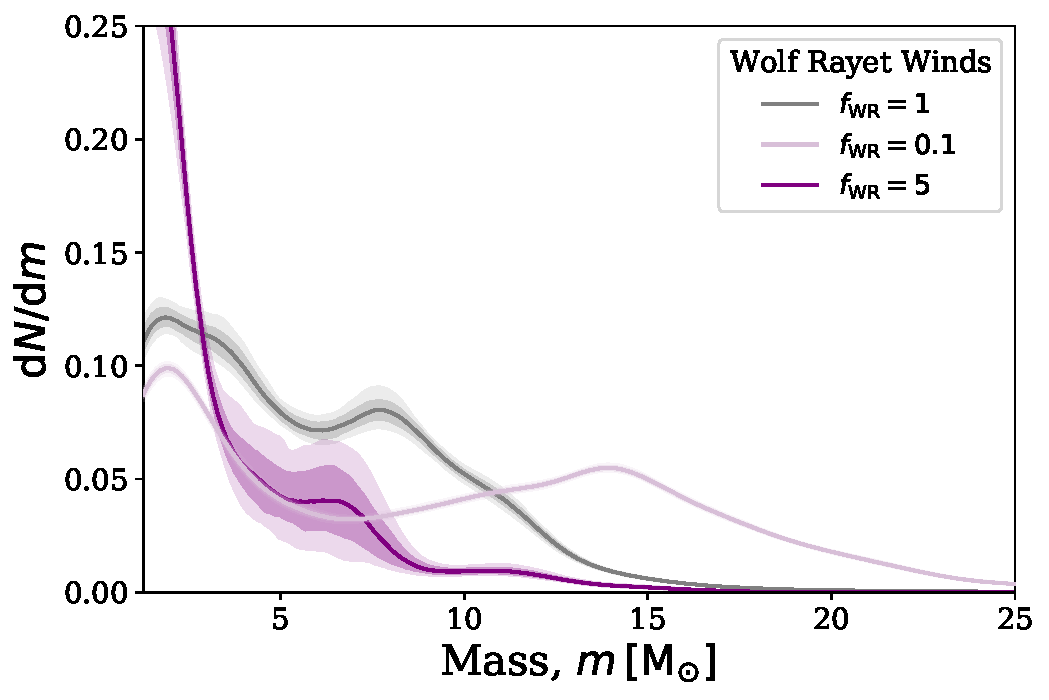
\includegraphics[width=\columnwidth]{wr_wind_mass_variations.pdf}
    \caption{As Fig.~\ref{fig:lower_mass_gap_variation}, but instead varying Wolf-Rayet wind efficiency (models \modWRLow{} and \modWRHigh{}). \href{https://github.com/TomWagg/detecting-DCOs-in-LISA/blob/main/paper/figures/wr_wind_mass_variations.pdf}{\faFileImage} \href{https://github.com/TomWagg/detecting-DCOs-in-LISA/blob/main/paper/figure_notebooks/variations.ipynb}{\faBook}.}
    \label{fig:wr_wind_mass_variations}
\end{figure}

In Fig.~\ref{fig:wr_wind_mass_variations} we show the effect that changing the efficiency of Wolf-Rayet winds has on the individual component mass distribution. Decreasing the Wolf-Rayet wind efficiency allows the formation of more massive DCOs in the Milky Way and, indeed, we see that the distribution extends to $25 \unit{M_{\odot}}$ and fewer detectable systems are formed at low masses. By contrast, increasing the Wolf-Rayet efficiency by a factor of 5 strongly disfavours the formation of systems at high masses and approximately 85\% of detectable systems have masses below $5 \unit{M_{\odot}}$. These three distributions are very distinct and so it is possible that the mass distribution of LISA could help to constrain the efficiency of Wolf-Rayet winds.
